
\documentclass[a4paper,11pt]{report}

\usepackage{amsmath}
\usepackage{amssymb}
\usepackage[utf8x]{inputenc}
\usepackage{fullpage}
\usepackage[hyphens]{url}
%\usepackage{hyperref} %this messes up the line breaks of url
\usepackage{xspace}
\usepackage{graphicx}
\usepackage{longtable}
\usepackage{subcaption}
\usepackage{listings}

%%commands
\newcommand{\sname}{QRSim\xspace}
\newcommand{\snamettt}{\texttt{QRSim}\xspace}

\newcommand{\webrepo}{\url{http://complacs.cs.ucl.ac.uk/complacs/simulator/qrsim-lastStable.zip}\xspace}
\newcommand{\webman}{\url{http://complacs.cs.ucl.ac.uk/complacs/simulator/manual.pdf}\xspace}

\newcommand\mytexttt[1]{\texttt{\hyphenchar\font=45\relax #1}}
\newcommand{\nn}{\nonumber}
\newcommand{\pr}{{\rm Pr}}


% Title Page
\title{{CompLACS} Helicopters Scenarios}
\author{\bf PRELIMINARY VERSION}
%\author{Renzo De Nardi,\\University College London\\\texttt{rdenardi@cs.ucl.ac.uk}}

\begin{document}
\maketitle



\begin{abstract}
This document describes the three types of scenarios devised at UCL to develop and test learning and control algorithm with application to a flock of autonomous quadrotor helicopters, one of the three real world platforms of the {CompLACS} project.
The three application scenarios are explicitly chosen to expose different types of challenges that occur in the domain of multi-platform aerial robotics so to provide a variety of research opportunities.

This report is divided into three parts one for each of the three scenarios; each part gives a formal description of the scenario in terms of its setup, its objective, and its variations. 

In order to aid the development and testing of learning algorithms, we provide a simulation environment based on the \sname quadrotor simulator for each the scenarios along with handy code examples.
Technical details specific to the scenarios implementation are reported in the appendix. 

Since the scenarios simulations are built on top of our \sname, we refer to the \sname manual (\webman) for details about the simulator and its API.

\end{abstract}

\tableofcontents

\chapter{Scenario 1: Cats and Mouse game}

The first of the scenarios is designed to focus primarily on the challenges encountered in the coordinated control of multiple UAVs; the associated problems of sensing and state estimation are somewhat simplified by the choice of task, environment and platform sensors. 

\section{Description}
The task to be accomplished in this scenario is in the form of a team game in which $N$ helicopters (cats) have to surround and effectively trap (i.e. get close to) another helicopter (mouse) at the end of the allotted time. 

For simplicity the task is assumed to take place in an area devoided of obstacles so that helicopters can fly freely. The platforms are equipped with noisy sensors so only observation of the vehicle state are available.  
It is assumed that each helicopter has also timely access to observations of the location and velocity of all the other platforms. 
Depending on the circumstances in the flight area there might be present wind and other aerodynamic disturbances that affect the flight behaviour of the platforms.

Snapshots of the initial ($t=0$) and terminal($t=T$) configurations from a typical successful run are visible in figures \ref{fig:catmousestart} and \ref{fig:catmousestop} respectively. 

In the next section we give a more formal description of the problem.

\begin{figure}[h]
\centering
\subcaptionbox{$t=0$\label{fig:catmousestart}}{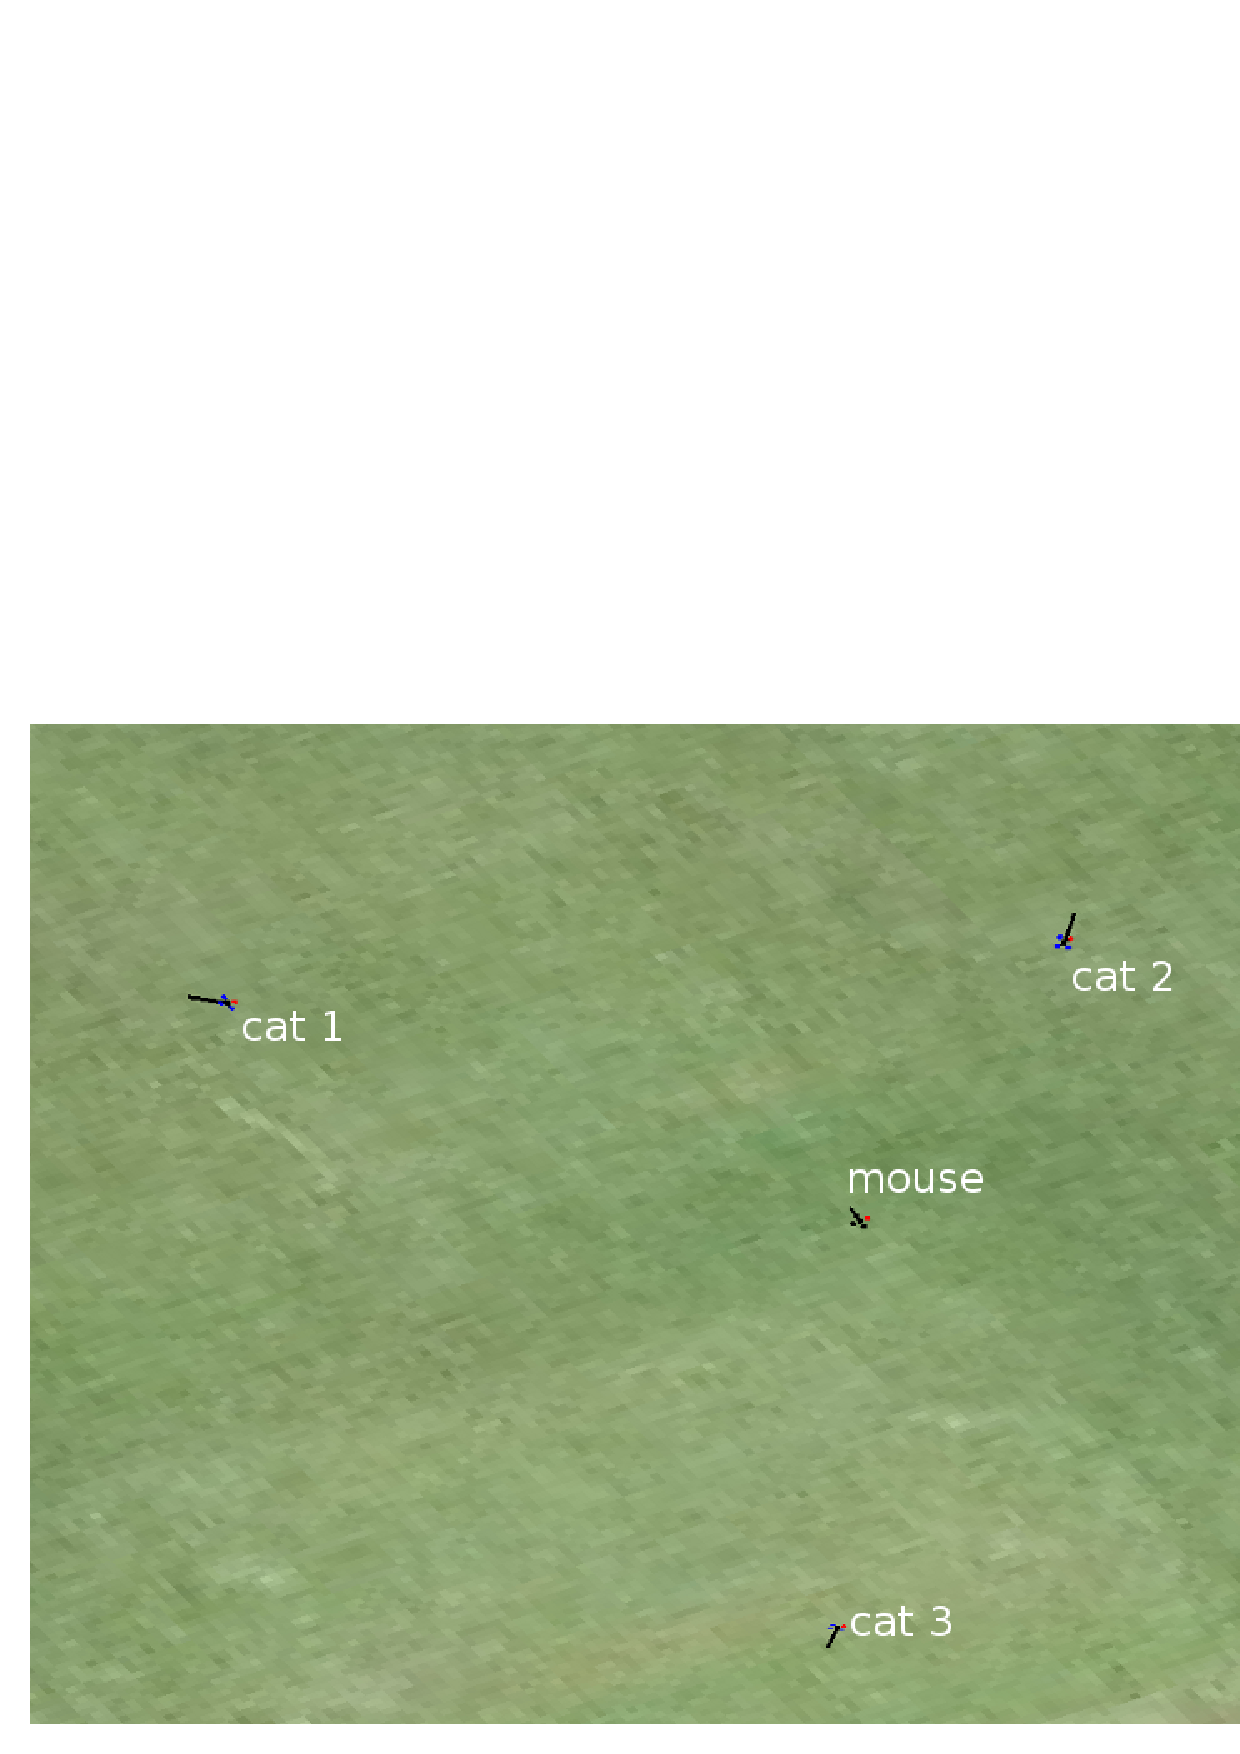
\includegraphics[width=0.49\textwidth]{catmousestart.jpg}}
\subcaptionbox{$t=T$\label{fig:catmousestop}}{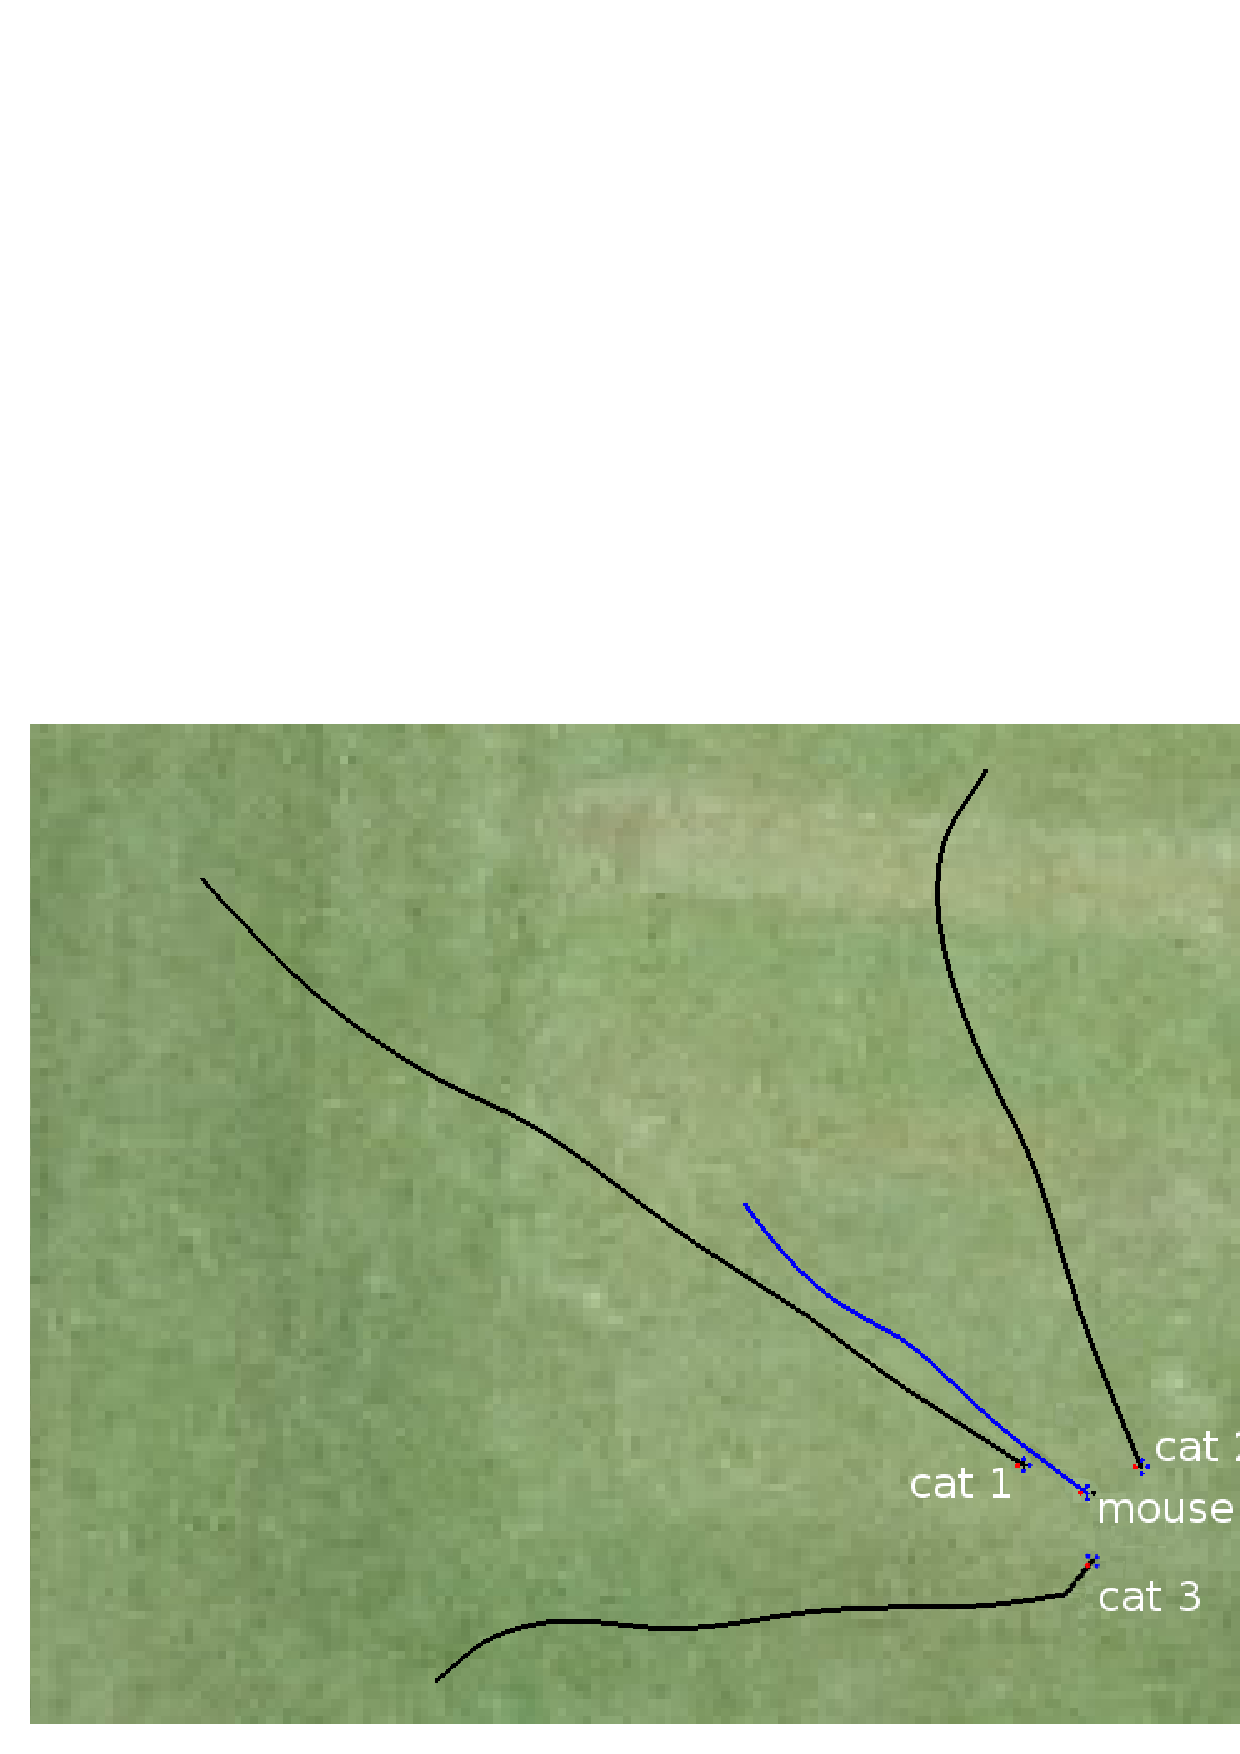
\includegraphics[width=0.49\textwidth]{catmousestop.jpg}}
\caption{Typical successful run: start(a) and end(b) configurations. \label{fig:catmouse}}
\end{figure}

\section{MDP}

The underlying system is modelled as a discrete time, finite horizon MDP on a continuous state space. The system runs from $t=0$ to $t=T$ with a time step equivalent to $1s$ of simulated time\footnote{The update rate is user-configurable with default value of 1Hz.}. 

\paragraph{States:} The state $s_t = (x^1_t,...,x^{N}_t,x^m_t)$ at time $t$ comprises of the state vectors of all the cats (superscripts $1,...,N$) and of the mouse (superscript $m$) helicopters. 
Each platform state contains in turn the position ($[p_x,p_y,p_z]^\intercal$), velocity ($[u,v,w]^\intercal$), orientation ($[\phi,\theta,\psi]^\intercal$) and rotational velocity ($[p,q,r]^\intercal$) of the platform. All of these are continuous variables (see section \ref{CatMouseSim} for more details).

The environment is itself three dimensional although we will see (section \ref{catmouseactions}) that the helicopters are assumed to fly at a fixed altitude.

\paragraph{Initial State:} At the beginning of the task the mouse is placed at the center of the flight space\footnote{Without loss of generality since the control problem depends on the relative positions of mouse and cats as long as the flying area is sufficiently large.} and the cats are positioned randomly around the mouse.

The initial position of cats are generated as:
$$
\left\{
\begin{array}{l l}
p^i_x =  d_i \cos(\alpha_i) & \\
p^i_y =  d_i \sin(\alpha_i) & i \in 1..N\\
p^i_z = - h_{fix} & \\
\end{array}
\right.
$$
where $\alpha_i \in \mathcal{U}(0,2\pi)$, $d_i \in \mathcal{U}(D_m,D_M)$ and $\mathcal{U}(a,b)$ indicates a uniform distribution over the interval $[a,b]$. The minimum and maximum distance from the mouse $D_m,D_M$ and the altitude $h_{fix}$ are user-configurable.
An additional parameter $D_{c2c}$ allows to define a minimum distance between any two cats; this prevent the occurrence of an initial state in which two cats are too close.

At $t=0$ all the helicopters are stationary (i.e. their velocities are zero).

\paragraph{Actions:}\label{catmouseactions} 
A real quadrotor of the type considered in our task generally presents four continuous control inputs (i.e. pitch, roll, yaw angles and throttle) which needs to be updated at a rate of $50Hz$, constituting a rather large control space.

To limit the space of control inputs, in our setup each UAV is equipped with a close loop PID controller that accepts 2D linear velocity commands $a^i_t=[v^i_x,v^i_y,v^i_z]^\intercal$ (in global coordinates) and combines them with the estimated platform velocity to produce the necessary attitude and throttle commands for the platform. The PID accepts commanded velocity at a rate of $1Hz$ and provides the platform controls at $50Hz$.
To additionally reduce the control space the PID takes also care of maintaining a constant altitude and heading\footnote{The use of a PID controller in addition to reducing the number of control inputs makes the task closer to what is possible to implement and test using real quadrotors.}. 

The action space $a_t = (a^1_t,...,a^{N}_t)$ at time $t$ comprises of the 2D linear velocity commands for each of the cats helicopters. 

\paragraph{Dynamics:} 
Markovian transition dynamics are defined by a distribution $P(s_{t+1}|s_t,a_t)$ which denotes the conditional density of state $s$ at time $t+1$ given state-action $(s_t,a_t)=(s,a)$ at time~$t$.

In the case of the cats helicopters the transition dynamics is defined by the combination of PID velocity controllers, platforms dynamics, sensor and wind dynamics (since these in turn effect the quadrotor) all of which are part of the \sname simulator\footnote{We refer to the \sname manual \webman for details.}. 

For the mouse helicopter the transition dynamics is 
not only defined by the platform dynamics but also by the way the mouse moves in response to the cats. 
 As the task starts the mouse helicopter tries to escape the cats by moving at a constant (max) speed\footnote{While the control law that governs the quadrotor attempts to maintain a fix maximum speed, in practice the true speed will not be constant due to sensor noise wind disturbance and dynamic effects.} and choosing a direction that prioritize escaping from the closer cats.
In specific the 2D velocity action for the mouse at time $t$ is computed as:
\begin{equation}\label{eqn:mousectrl}
\begin{array}{ll}
a^m_t = V_{M} \frac{\mathsf{v}_t}{\| \mathsf{v}_t \|} &
\text{where } \;\;\mathsf{v}_t = \sum_{i=1}^N \frac{\left[\begin{array}{c} p^i_x \\ p^i_y \end{array}\right]_t - \left[\begin{array}{c} p^m_x \\ p^m_y \end{array}\right]_t}{\left\| \left[\begin{array}{c} p^i_x \\ p^i_y \end{array}\right]_t - \left[\begin{array}{c} p^m_x \\ p^m_y \end{array}\right]_t \right\|^2}
\end{array}
\end{equation}
and $V_{M}$ is the (user-configurable) maximum speed that the mouse can achieve. 

Different control strategies could be considered for the mouse; in practise the one considered in equation \ref{eqn:mousectrl} is both simple and has shown to be sufficient to provide for a challenging task.


\paragraph{Rewards:}
The cats are successful if the are able to trap the mouse at the end of the task; a meaningful final reward can be defined as the sum of the squared (2D) distances\footnote{$d_{2D}(x^i_T,x^m_T) = \Vert[p^i_x,p^i_y]_T^\intercal - [p^m_x,p^m_y]_T^\intercal\Vert$.} between the cats and the mouse at time $T$:
$$r_T = - \sum^N_{i=1} d_{2D}(x^i_T,x^m_T)^2.$$
A large negative reward\footnote{The default value of the negative reward is $-1000$ but it can be configured by the user.} is returned if any of the helicopters (including the mouse) goes outside of the flying area or if any collision happens during the task.

\section{Task Variations} \label{CatMouseVariations}
The difficulty of the considered control problem depends on the level of sensor noise and wind disturbance; so we define three versions of the task with increasing level of realism (and consequently difficulty):
\begin{itemize}
 \item \textit{\textbf{1A} noiseless:} the dynamics of the quadrotors is deterministic and the state returned is the true platform state;
 \item \textit{\textbf{1B} noisy:} the dynamics of the quadrotors is stochastic and the state returned is a noisy estimate of the platform state (i.e. with additional correlated noise);
 \item \textit{\textbf{1C} noisy and windy:} the dynamics of the quadrotors is stochastic and affected by wind disturbances (following a wind model), the state returned is a noisy estimate of the platform state (i.e. with additional correlated noise).
\end{itemize}

%If there is sufficient interest additional variations could be added, these includes (but are not limited to):
%\begin{itemize} 
%\item \textit{obstacles:} e.g. cylinders in the flying area which are impassable and result in crashes. The obstacles would be represented by providing the coordinates of their center and radius, for example.
%\item \textit{multitask:} a multitask setting which involves repeated attempts at tasks drawn from some distribution.
%\end{itemize}

\section{Simulation Code}\label{CatMouseSim}
The cat and mouse scenario can be promptly defined on top of the \sname simulator by means of dedicated task classes\footnote{We refer to the \webman for details on task classes.}. In specific we make available one task class for each of the three scenario variations introduced in section \ref{CatMouseVariations}:
\begin{itemize}
\item\textit{1A}: \mytexttt{TaskCatsMouseNoiseless.m},
\item\textit{1B}: \mytexttt{TaskCatsMouseNoisy.m},
\item\textit{1C}: \mytexttt{TaskCatsMouseNoisyAndWindy.m}. 
\end{itemize}

Commenting the code in details is beyond the scope of this report but it is useful to briefly report which task methods are responsible for handling the various task specific definitions:
\begin{itemize}
\item\mytexttt{init()}: defines all the platforms and sensor parameters;
\item\mytexttt{reset()}: defines the task starting condition;
\item\mytexttt{step(U)}: defines the mouse evasion strategy;
\item\mytexttt{reward()}: defines the task reward.
\end{itemize}

Listing \ref{lst:mcm} (file \texttt{main\_catsmouse.m}) shows the set of steps that are necessary to run a scenario task.

After the desired task is initialized (line 4), a basic for loop is executed for the number of timesteps specified by the task. Within the loop the 2D velocity control is computed for each helicopter and passed to the corresponding PID (line 37). 
In our listing we show a simple (and suboptimal) scheme in which the velocity direction of each cat directly towards the future mouse position mouse (line 20-23) but that also keeps away from neighbouring cats (line 26-34). 
The helicopter control input produced by the PID controllers are then used to step the simulator (line 41).
Finally after the execution of the task is concluded, the final reward for the task can be retrieved (line 46).

We remind the reader that within the simulator the helicopter state $x^i$ is denoted as \texttt{eX}:
$$\texttt{eX} = [\tilde{p}_x,\tilde{p}_y,\tilde{p}_z,\tilde{\phi},\tilde{\theta},\tilde{\psi},0,0,0,\tilde{p},\tilde{q},\tilde{r},0,\tilde{a}_x,\tilde{a}_y,\tilde{a}_z,h,\dot{p}_x,\dot{p}_y,\dot{h}]^\intercal$$
while the actions $a^i$ are denoted as controls \texttt{u}:
$$\texttt{u}=[v_x,v_y]^\intercal$$
with the variables defined in section \ref{tab:naming}.

\begin{lstlisting}[float=ht!bp,caption=main\_catsmouse.m,language=Matlab,frame=lines,label=lst:mcm,numbers=left,basicstyle=\small]
qrsim = QRSim();

% load task parameters and do housekeeping
state = qrsim.init('TaskCatsMouseNoisyAndWindy');

U = zeros(2,state.task.Nc);

% run the scenario and at every timestep generate a control
% input for each of the uavs
for i=1:state.task.durationInSteps,
    
    % get the mouse position (note id state.task.Nc+1)
    mousePos = state.platforms{state.task.Nc+1}.getEX(1:2);
    
    % quick and easy way of computing velocity controls for each cat 
    for j=1:state.task.Nc,
	collisionDistance = state.platforms{j}.getCollisionDistance();
		
        % vector to the mouse
        u = mousePos - state.platforms{j}.getEX(1:2);
        
        % add a weighted velocity (i.e. "predict" where the mouse will be)
        u = u  + (norm(u)/2)*state.platforms{state.task.Nc+1}.getEX(18:19);
        
        % keep away from other cats if closer than 2*collisionDistance        
        for k = 1:state.task.Nc,
            if(state.platforms{k}.isValid())                  
                d = state.platforms{j}.getEX(1:2) 
                    - state.platforms{k}.getEX(1:2);
                if((k~=j)&&(norm(d)<2*collisionDistance))
                    u = u + (1/(norm(d)-collisionDistance()))*(d/norm(d));
                end
            end
        end
        
        % scale by the max allowed velocity
        U(:,j) = state.task.velPIDs{j}.maxv*(u/norm(u));
    end
    
    % step simulator
    qrsim.step(U);
end

% get final reward
fprintf('final reward: %f\n',qrsim.reward());

\end{lstlisting}

The task, the configurations and the example main files are in the directory \mytexttt{scenarios/catsmouse} within the \sname simulator. 

\newpage
\chapter{Scenario 2: Search and Rescue}
The second scenario is designed explicitly to expose the complex interplay between sensing and acting typical in autonomous robotics task. To solve the task the agent/s has to perform inference about the state of the environment given some observations and take actions based on its belief. 

\section{Description}
The task to be accomplished in this scenario is in the form of a wilderness search and rescue mission; several targets (people) are lost/injured on the ground in a landscape and need to be located and rescued. 

In addition to its navigation sensors each helicopter agent taking part in the search 
is equipped with a camera/classification module that allows it to detect the presence of targets in its field of view. Rather than raw images the camera module provides higher-level data in the form of log likelihood differences for the current observation conditioned on the presence or absence of a target. The quality of detection depends upon the ground type and the geometry between helicopter and ground (e.g. the distance). 

The search era is limited but its extent is so that a trivial lawn mower pattern of search will not allow to cover all the area in the allotted time. The landscape has different types of terrain; persons are more likely to be present on some class of terrain than others. For simplicity the persons are assumed to not move during the task. 

A snapshot from a typical run is shown in figure \ref{fig:searchrescue} along with an example of the observation returned by the camera/classifier model.
\begin{figure}[h]
\centering
\includegraphics[width=16cm]{searchrescue.jpg}
\caption{Search and rescue run with three helicopters; note the different terrain types (denoted by different colors) and the persons (red dots). The insert shows the camera observation from UAV 1 that happens to be over a person. \label{fig:searchrescue}}
\end{figure}

\section{MDP}
The underlying system is modelled as a discrete time, finite horizon MDP on a continuous state space. The system runs from $t=0$ to $t=T$ with a time step equivalent to $1s$ of simulated time\footnote{The update rate is user-configurable with default value of 1Hz.}.

\paragraph{States:} the state $s_t=(x^1_t,...,x^{N}_t,b^i_t,...,b^P_t)$ at time $t$ comprises the helicopters state vectors $x^i_t$ and the position of  the targets 


which includes the agents position, velocity and orientation, and $b^i_{t}$, for $i\in\{1,...,P\}$ the position of $P$ targets. All are continuous variables. We assume that the ground is flat and that the targets are located on the ground.


{States:} The state $s_t = (x^1_t,...,x^{N}_t,x^m_t)$ at time $t$ comprises of the state vectors of all the cats (superscripts $1,...,N$) and of the mouse (superscript $m$) helicopters. 
Each platform state contains in turn the position ($[p_x,p_y,p_z]^\intercal$), velocity ($[u,v,w]^\intercal$), orientation ($[\phi,\theta,\psi]^\intercal$) and rotational velocity ($[p,q,r]^\intercal$) of the platform. All of these are continuous variables (see section \ref{CatMouseSim} for more details).

The environment is itself three dimensional although we will see (section \ref{catmouseactions}) that the helicopters are assumed to fly at a fixed altitude.


\paragraph{Dynamics:} Markovian transition dynamics for the helicopter\footnote{We refer to the \sname manual \webman for detail about the helicopter transition dynamics.} are defined by $P(x_{t+1}|x_t,a_t)$ which denotes the conditional density of state $x$ at $t+1$ given $(x_t,a_t) = (x,a)$ at time $t$. These dynamics are independent of the targets $b^i_t$.

Targets $b^i_t$ are stationary unless a helicopter hovers (i.e. its speed is low) sufficiently close to it, in which case the target is removed from the environment.
More formally:
\begin{align}
if ~ \exists ~ i~:~ d_{3D}\left( x_t,b^i_t \right) < \delta ~ \wedge ~\and \parallel [u,v,w]_t^\intercal \parallel < \epsilon \quad \Rightarrow \quad N=N-1\qquad i\in\{1,...,N\}
\end{align}
where $d_{3D}$ is the standard Euclidean distance\footnote{Defined as $$d_{3D}(x_t,b^i_t) = \parallel b^i_t -[p_x,p_y,p_z]_t^\intercal \parallel.$$} and $(\epsilon,\delta)$ are user specified thresholds\footnote{The default values for the distance threshold and the speed threshold are $\delta=5m$ and $\epsilon=0.1m/s$}.

\paragraph{Actions:}
the action $a_t$ at time $t$ is expressed in terms of a 3D velocity vector in global NED coordinates:
\begin{align}
a_t=[v_x,v_y,v_z]_t^\intercal.
\end{align}
Is worth remembering that the actions are nothing more than set points to a PID controller that attempts to drive that UAV at the requested velocity.
Due to delays and disturbances mismatches between the commanded and the actual velocity of the UAV have to be expected.

\paragraph{Rewards:} 
According to the way a target is rescued the reward $r_t$ at time $t$ is defined to be $1$ when a helicopter hovers sufficiently close to a target and a small negative value otherwise.
More formally:
\begin{align}
r_t =  \left\{
\begin{array}{c l}
1 & if ~ \exists ~ i~:~ d_{3D}\left( x_t,b^i_t \right) < \delta ~ \wedge ~\and \parallel [u,v,w]_t^\intercal \parallel < \epsilon \qquad i\in\{1,...,N\}\\
-1/T & otherwise
\end{array}
\right.
\end{align}
for a task duration $T$ and the same $\epsilon,\delta$ that define a person as rescued. 
A large negative reward\footnote{The default value of the negative reward is $-1000$ but it can be configured by the user.} is returned if the helicopter goes outside of the flying area or if any collision happens during the task. 

\section{Observations}

The helicopter state $x_t$ is observed directly although depending on the specific task variation (see Section~\ref{SearchRescueVariations}) the state variables might be affected by stochastic noise.

The position of the targets $b^i_t$ is not known, but observations $o_t$ are provided by the camera at each time step.

Following standard object detection techniques we assume that the incoming image is split into $M$ windows $\{w^j_t\}^M_{j=1}$  (of size informed by the current altitude and an assumed fixed size for the person) which are then analysed for targets. 
Given the current UAV pose $x_t$ and the fixed camera parameters the set of windows re-projects to a set of $M$ patches $\{g^j_t\}^M_{j=1}$ on the ground\footnote{Here we assume that everything needed to provide the link between the ground coordinates and the camera's frame is engineered by hand and does not have to be learned autonomously. In other words it is assumed that a map is available and known and the mapping
\begin{align}
\{g^j_t\}^M_{j=1} \mapsto \{w^j_t\}^M_{j=1}\nn
\end{align}
is known, but does not have to be considered explicitly by the agent.} with centres $\{c^j_t\}^M_{j=1}$.
The observation $o_t$ is simply the collection of the log likelihood ratios for each of the ground patches $g^j_t$:
\begin{align}
o_t = \left\{\log
\left(
\frac{\pr(\mbox{image at time } t~|~\mbox{target in } g^j_t \mbox{, agent at }x_t)}
{\pr(\mbox{image at time }t~|~\mbox{no target in } g^j_t \mbox{, agent at }x_t)}
\right)
\right\}^M_{j=1}. \nn
\end{align}


\section{Task Variations} \label{SearchRescueVariations}
The difficulty of solving the task depends on the number of platforms that are employed as well as on the level of sensor noise and wind disturbance; we provide four versions of the task with increasing level of difficulty:
\begin{itemize}
 \item \textit{\textbf{2A} single helicopter noiseless:} only one helicopter is used for the search, its dynamic is deterministic and the state returned is the true platform state;
 \item \textit{\textbf{2B} single helicopter noisy:} only one helicopter is used for the search, its dynamics is stochastic and the state returned is a noisy estimate of the platform state (i.e. with additional correlated noise);
 \item \textit{\textbf{2C} multiple helicopters noiseless:} several helicopters are used for the search, their dynamics is deterministic and the state returned is the true platform state;
 \item \textit{\textbf{2D} multiple helicopters noisy and windy:} several helicopters are used for the search, their dynamics is stochastic and affected by wind disturbances (following a wind model), the state returned is a noisy estimate of the platform state (i.e. with additional correlated noise).
\end{itemize}

\section{Simulation Code} \label{SearchRescueSim}

All the ingredients of the scenario described above are implemented as task classes for the \sname quadrotor simulator; the four variations of the scenario are named:
\begin{itemize}
\item\textit{2A}: \mytexttt{TaskSearchRescueSingleNoiseless.m}, 
\item\textit{2B}: \mytexttt{TaskSearchRescueSingleNoisy.m}, 
\item\textit{2C}: \mytexttt{TaskSearchRescueMultipleNoiseless.m} 
\item\textit{2D}: \mytexttt{TaskSearchRescueMultipleNoisyAndWindy.m}. 
\end{itemize}

We also provide the example file \texttt{main\_searchrescue.m} which shows how to initialize and run a task, how to retrieve the platform state, retrieve the observations and issue actions.

The task, the configurations and the example main files are in the directory \mytexttt{scenarios/searchrescue} within the \sname simulator. 

\textbf{Note:}
Within the simulator the helicopter state $x^i$ is denoted as $eX$:
$$eX = [\tilde{p}_x,\tilde{p}_y,\tilde{p}_z,\tilde{\phi},\tilde{\theta},\tilde{\psi},0,0,0,\tilde{p},\tilde{q},\tilde{r},0,\tilde{a}_x,\tilde{a}_y,\tilde{a}_z,h,\dot{p}_x,\dot{p}_y,\dot{h}]^\intercal$$
while the actions $a^i$ are denoted as controls $u$:
$$u=[v_x,v_y,v_z]^\intercal$$
with the variables defined in appendix \ref{tab:naming}.

\newpage
\chapter{Scenario 3: Plume modelling}


\section{Description}
Several smoke plumes evolve over time and a helicopter agent is equipped with a sensor that measures the concentration of smoke. The plume follows a known model but with unknown parameter values. The objective is to provide a smoke concentration estimate $\hat{c}_T$ at some pre-specified time $T$\footnote{For simplicity we refer to concentration of smoke, in a real environment this would be a property of the plume that can be realistically measured e.g. CO concentration.}.


\begin{figure}[h]
\centering
\subcaptionbox{Single source Gaussian concentration.\label{fig:singlegaussplume}}{\includegraphics[width=0.49\textwidth]{singlegaussplume.jpg}}
\subcaptionbox{Multiple sources Gaussian dispersion.\label{fig:multigaussplume}}{\includegraphics[width=0.49\textwidth]{multigaussplume.jpg}}
\subcaptionbox{Single source Gaussian puff dispersion.\label{fig:singlegausspuffplume}}{\includegraphics[width=0.49\textwidth]{singlegausspuffplume.jpg}}
\caption{Plume models.\label{fig:plume}}
\end{figure}

\section{MDP}
The underlying system is modelled as a discrete time Markov process on a continuous state space. The system is updated at a frequency of 1Hz\footnote{The update rate is user-configurable with default value of 1Hz.}. 

\paragraph{States:} the state $s_t=(x_t,c_t)$ at time $t$ comprises the helicopter data $x_t$ which includes the agents position, velocity and orientation, which are continuous variables, and $c_t$ the smoke concentration over the whole flight volume, also continuous.

\paragraph{Actions:}
The action $a_t$ at time $t$ is expressed in terms of a velocity vector in global NED coordinates:
\begin{align}
a_t=[v_x,v_y,v_z]_t^\intercal.
\end{align}

\paragraph{Dynamics:} Markovian transition dynamics for the helicopter\footnote{We refer to the \sname manual \webman for detail about the helicopter transition dynamics.} and the smoke concentration are defined by $P(s_{t+1}|s_t,a_t)$ which denotes the conditional density of state $s$ at $t+1$ given $(s_t,a_t) = (s,a)$ at time $t$. The smoke evolves according to a plume model (see section \ref{PlumeVariations} for details) and its evolution is assumed to be independent of the helicopter actions and state  $P(c_{t+1}|c_t,x_t,a_t)=P(c_{t+1}|c_t)$.

\paragraph{Observations:} The helicopter state $x_t$ is observed directly although depending on the specific task variation (see Section~\ref{PlumeVariations}). 
The smoke concentration $c_t$ is not known, but noisy observations $o_t$ are provided by a concentration sensor at each time step returning the concentration at the position in which the helicopter is located.

\paragraph{Reward:} 
For the tasks 3A, 3B, 3C and 3D (see section \ref{PlumeVariations}) in which the concentration is static, the agent must provide a set of concentration estimates $\{\hat c^j_T\}^M_{j=1}$ at a series of $M$ spatial locations specified by the task. 
Given the $\{\hat c^j_T\}^M_{j=1}$ the performance is simply computed as (minus) the square error between the true concentrations and the estimates provided by the agent:
$$
r_T = - \sum^M_{j=1} | c^j_T - \hat{c}^j_T |^2 .
$$

For tasks 3E, 3F and 3G in which the concentration evolves in time, each $\hat c^j_T$ can be though of as a random variable with an associated probability distribution $\pr(\hat c^j_T)$.
The performance is computed as the KL divergence from the true concentration distribution\footnote{In practice in order to enable the computation of the reward the agent will be asked to repeatedly return (i.e. draw samples from its distribution) the value of $\hat c_t$ at the locations specified by the task.} $\pr(c_T)$ and the provided estimate $\pr(\hat c_T)$:
$$
r_T = KL(\pr(c^1_T,..,c^M_T) \|{\pr}(\hat c^1_T,..,\hat c^M_T)).
$$

\section{Task Variations}  \label{PlumeVariations}
The complexity of the estimation problem changes substantially depending on the type of dispersion model followed by the plume, and on the number of helicopters used to tackle the task hence we provide several version of the task with increasing level of difficulty:
\begin{itemize}
\item \textit{\textbf{3A} single source static Gaussian concentration:} only one helicopter is used for the sampling, its dynamic is deterministic, the state returned is the true platform state, the smoke concentration is static and has the form or a three dimensional Gaussian centred at the source (see equation \ref{eqn:singlesourcegaussian}).

\item \textit{\textbf{3B} single source static Gaussian dispersion model:} only one helicopter is used for the sampling, its dynamics is stochastic and affected by wind disturbances (following a wind model), the state returned is a noisy estimate of the platform state (i.e. with additional correlated noise) and the smoke concentration is static and has the form specified by what is commonly called a Gaussian dispersion model (see equation \ref{eqn:singlesourcegaussiandispersion}).

\item \textit{\textbf{3C} multiple sources static Gaussian dispersion model:} only one helicopter is used for the sampling, its dynamics is stochastic and affected by wind disturbances (following a wind model), the state returned is a noisy estimate of the platform state (i.e. with additional correlated noise) and the smoke concentration is static and has the form specified by the superposition of several sources each of which follows a Gaussian dispersion model (see equation \ref{eqn:multiplesourcesgaussiandispersion}).

\item \textit{\textbf{3D} multiple helicopters multiple sources static Gaussian dispersion model :} as above but multiple helicopters are used for the sampling.

\item \textit{\textbf{3E} single source time-varying Gaussian puff dispersion model:} only one helicopter is used for the sampling, its dynamics is stochastic and affected by wind disturbances (following a wind model), the state returned is a noisy estimate of the platform state (i.e. with additional correlated noise) and the smoke concentration is time-varying and has the form specified by what is commonly called a Gaussian puff dispersion model (see equation \ref{eqn:singlesourcesgaussianpuffdispersion}).

\item \textit{\textbf{3F} multiple sources time-varying Gaussian puff dispersion model:} only one helicopter is used for the sampling, its dynamics is stochastic and affected by wind disturbances (following a wind model), the state returned is a noisy estimate of the platform state (i.e. with additional correlated noise) and the smoke concentration is static and has the form specified by the superposition of several sources each of which follows a Gaussian puff dispersion model (see equation \ref{eqn:multiplesourcesgaussianpuffdispersion}).

\item \textit{\textbf{3G} multiple helicopters multiple sources time-varying Gaussian puff dispersion model :} as above but multiple helicopters are used for the sampling.

\end{itemize}

\textit{Note:}
Since the dispersion models are known, one possible way to solve the tasks is to estimate the model parameters (or a distributions over them); while this is an appropriate solution we emphasize that the agent is not required to solve the task in this way and so other forms for the concentration (or for the distribution over the concentration) are equally appropriate.  

\section{Simulation Code} \label{PlumeSim}

All the ingredients of the scenario described above are implemented\footnote{We are currently in the process of finalizing the implementation.} as a task class for the quadrotor simulator \sname\footnote{We refer to the \sname manual for details on the simulator API \webman.}; the seven variations of the scenario are named:
\begin{itemize}
\item\textit{3A}: \mytexttt{TaskPlumeSingleSourceGaussian.m}, 
\item\textit{3B}: \mytexttt{TaskPlumeSingleSourceGaussianDispersion.m},
\item\textit{3C}: \mytexttt{TaskPlumeMultiSourceGaussianDispersion.m}, 
\item\textit{3D}: \mytexttt{TaskPlumeMultiHeliMultiSourceGaussianDispersion.m}, 
\item\textit{3E}: \mytexttt{TaskPlumeSingleSourceGaussianPuffDispersion.m}, 
\item\textit{3F}: \mytexttt{TaskPlumeMultiSourceGaussianPuffDispersion.m},
\item\textit{3G}: \mytexttt{TaskPlumeMultiHeliMultiSourcePuffDispersion.m}. 
\end{itemize}

We also provide the example file \texttt{main\_plume.m} which shows how to initialize and run a task, how to retrieve the platform state, retrieve the observations, retrieve the location at which to provide estimates, issue actions and return concentration estimates.

The task, the configurations and the example main files are in the directory \mytexttt{scenarios/plume} within the \sname simulator. 

\textbf{Note:}
Within the simulator the helicopter state $x^i$ is denoted as $eX$:
$$eX = [\tilde{p}_x,\tilde{p}_y,\tilde{p}_z,\tilde{\phi},\tilde{\theta},\tilde{\psi},0,0,0,\tilde{p},\tilde{q},\tilde{r},0,\tilde{a}_x,\tilde{a}_y,\tilde{a}_z,h,\dot{p}_x,\dot{p}_y,\dot{h}]^\intercal$$
while the actions $a^i$ are denoted as controls $u$:
$$u=[v_x,v_y,v_z]^\intercal$$
with the variables defined in section \ref{tab:naming}.

\newpage

\appendix

\chapter{Nomenclature}\label{tab:naming}

Helicopter state variables common to all the tasks:
\begin{table}[h]  
\begin{tabular}{l l l}
     $p_x$ & true x position (NED coordinates)            & $m$\\
     $p_y$ & true y position (NED coordinates)            & $m$\\
     $\tilde{p}_x$ & x position estimate from GPS (NED coordinates)            & $m$\\
     $\tilde{p}_y$ & y position estimate from GPS (NED coordinates)            & $m$\\
     $\tilde{p}_z$ & z position estimate from GPS (NED coordinates)            & $m$\\
     $\tilde{\phi}$ & roll attitude in Euler angles right-hand ZYX convention & $rad$\\
     $\tilde{\theta}$ & pitch attitude in Euler angles right-hand ZYX convention& $rad$\\
     $\tilde{\psi}$ & yaw attitude in Euler angles right-hand ZYX convention  & $rad$\\
     $\tilde{p}$  & rotational velocity around x body axis from gyro                 & $rad/s$\\ 
     $\tilde{q}$  & rotational velocity around y body axis from gyro                 & $rad/s$\\ 
     $\tilde{r}$  & rotational velocity around z body axis from gyro                & $rad/s$\\
     $\tilde{a}_x$ & linear acceleration in x body axis from accelerometer            & $m/s^2$\\
     $\tilde{a}_y$ & linear acceleration in y body axis from accelerometer             & $m/s^2$\\
     $\tilde{a}_z$ & linear acceleration in z body axis from accelerometer             & $m/s^2$\\
     $h$& altitude\footnotemark  from altimeter NED & $m$\\
     $\dot{p}_x$ & x velocity from GPS (NED coordinates)            & $m/s$\\
     $\dot{p}_y$ & y velocity from GPS (NED coordinates)            & $m/s$\\
     $\dot{h}$    & altitude rate from altimeter NED                   & $m/s$\\
     $v_x$ & desired x velocity control (NED coordinates)            & $m/s$\\ 
     $v_y$ & desired y velocity control (NED coordinates)            & $m/s$\\
\end{tabular}
\end{table}

We remind the reader that NED stands for Noth-East-Down as explained in more detail in the \sname manual.

\newpage

\chapter{Concentration Models}

To interpret the following concentration models, is useful to introduce some nomenclature:
\begin{longtable}{l l l}
$x,y,z$ & coordinates w.r.t. the global NED frame of reference & $m$\\
$x',y',z'$ & coordinates w.r.t. the wind frame of reference & $m$\\
$X_s,Y_s$ & coordinates of the source w.r.t. the global NED frame  & $m$\\
$x\prime_s,y'_s$ & coordinates of the source w.r.t. the wind frame of reference  & $m$\\
$Q_s$ & emission rate of source $s$ & $Kg/s$\\
$H_s$ & equivalent height of source $s$ & $m$\\
$u$ & constant magnitude of the wind speed & $m/s$\\
$S$ & number of sources & \\
$a$ & diffusion parameter & $m^{2-b}$\\
$b$ & diffusion parameter & \\
$\alpha_w$ & wind direction (clockwise from north) & $rads$\\
$I_s$ & total number of puff for source $s$ & \\
$T^i_s$ & time at which puff $i$ of source $s$ was emitted & $s$\\
$Q^i_s$ & total amount of smoke emitted by source $s$ at time $T^i$ & $Kg$\\
$\boldsymbol\Sigma$ & Gaussian concentration covariance matrix \\
\label{tab:naming2}
\end{longtable}

We also introduce a change of reference frame, namely from global frame to wind frame (a frame of reference with origin in the global frame and aligned with the wind direction), since some of the models are expressed in this coordinates:
\begin{eqnarray}
x' &=& x \cos(\alpha_w) \\
y' &=& y \sin(\alpha_w).
\end{eqnarray}

\section{Single Source Gaussian Concentration Model}
\begin{equation}\label{eqn:singlesourcegaussian}
c(x,y,z) = %\frac{1}{(2\pi)^{3/2}|\boldsymbol\Sigma|^{1/2}}
\exp\left(-\frac{1}{2}
\left[\begin{array}{c}
x-X_s\\
y-Y_s\\
z-H_s
\end{array} \right]^T{\boldsymbol\Sigma}^{-1}
\left[\begin{array}{c}
x-X_s\\
y-Y_s\\
z-H_s
\end{array} \right]
\right)
\end{equation}

\section{Single Source Gaussian Dispersion Model}

A standard static plume dispersion (for more details see \cite{stockie2011}):
\begin{align}\label{eqn:singlesourcegaussiandispersion}
c(x',y',z) = &\frac{Q}{2\pi u a (x'-X'_s)^b}  \exp \left(-\frac{(y'-Y'_s)^2}{2 a (x'-X'_s)^b}\right) \nonumber \\
  & \left[ \exp \left(-\frac{(z-H_s)^2}{2 a (x'-X'_s)^b}\right) + \exp \left(-\frac{(z+H_s)^2}{2 a (x'-X'_s)^b}\right)\right].
\end{align}


\section{Multiple Sources Gaussian Dispersion Model}

In the case of multiple sources the total concentration can be computed by superposition:
\begin{align}\label{eqn:multiplesourcesgaussiandispersion}
c(x',y',z) = \sum_{s=1}^S c(x',y',z;X'_s,Y'_s,H_s,Q_s).
\end{align}

\section{Single Source Gaussian Puff Dispersion Model}

A standard time varying plume dispersion (for more details see \cite{stockie2011}):
\begin{align}\label{eqn:singlesourcesgaussianpuffdispersion}
c(x',y',z,t) = & \sum_{i=1}^I \left\{ \frac{Q^i_s}{8(\pi a (x'-X'_s)^b)^{3/2}} \right. \nonumber \\
& \exp\left(-\frac{(x'-X'_s-u(t-T^i_s))^2+(y'-Y'_s)^2}{2 a (x'-X'_s)^b}\right) \nonumber \\
& \left. \left[\exp\left(-\frac{(z-H_s)^2}{2 a (x'-X'_s)^b}\right) + \exp\left(-\frac{(z+H_s)^2}{2 a (x'-X'_s)^b}\right)\right]\right\}.
\end{align}

\section{Multiple Sources Gaussian Puff Dispersion Model}

Even in the case a time varying dispersion model, for multiple sources the total concentration can be computed by superposition:
\begin{align}\label{eqn:multiplesourcesgaussianpuffdispersion}
c(x',y',z,t) = \sum_{s=1}^S c(x',y',z,t;X'_s,Y'_s,H_s,Q^{1..I_s}_s).
\end{align}

\end{document}


